% options:
% thesis=B bachelor's thesis
% thesis=M master's thesis
% czech thesis in Czech language
% english thesis in English language

\documentclass[thesis=B,czech]{FITthesis}[2011/06/14]

\usepackage[utf8]{inputenc} % LaTeX source encoded as UTF-8

\usepackage{czech} % doplněno mnou

\usepackage{listings}
\lstloadlanguages{HTML, PHP, SQL, [LaTeX]TeX}
\renewcommand\lstlistingname{Ukázka kódu} % předefinování nadpisu
\renewcommand\lstlistlistingname{Ukázky zdrojových kódů}

\usepackage{graphicx} %graphics files inclusion
% \usepackage{amsmath} %advanced maths
% \usepackage{amssymb} %additional math symbols

% % list of acronyms
% \usepackage[acronym,nonumberlist,toc,numberedsection=autolabel]{glossaries}
% \iflanguage{czech}{\renewcommand*{\acronymname}{Seznam pou{\v z}it{\' y}ch zkratek}}{}
% \makeglossaries

\newcommand{\tg}{\mathop{\mathrm{tg}}} %cesky tangens
\newcommand{\cotg}{\mathop{\mathrm{cotg}}} %cesky cotangens

% % % % % % % % % % % % % % % % % % % % % % % % % % % % % % 
% ODTUD DAL VSE ZMENTE
% % % % % % % % % % % % % % % % % % % % % % % % % % % % % % 

\department{Katedra softwarového inženýrství}
\title{Systém pro daňovou evidenci krátkodobých akcí skautských organizací}
\author{František Hána} %jméno autora bez akademických titulů
\authorWithDegrees{František Hána} %jméno autora včetně akademických titulů
\supervisor{Mgr. Petr Matyáš}
\acknowledgements{Cht{\v e}l bych na tomto m{\' i}st{\v e} pod{\v e}kovat p{\v r}edev{\v s}{\' i}m m{\' e}mu vedouc{\' i}mu bakal{\' a}{\v r}sk{\' e} pr{\' a}ce Mgr. Petru Maty{\' a}{\v s}ovi za podporu p{\v r}i psan{\' i}, za p{\v r}ipom{\' i}nky a za metodick{\' e} veden{\' i} pr{\' a}ce. Také bych cht{\v e}l pod{\v e}kovat Ing. Ondřeji Pe{\v r}inovi za rady p{\v r}i psan{\' i} knihovny na komunikaci se syst{\' e}mem SkautIS.}
\abstractCS{
Bakal{\' a}{\v r}sk{\' a} pr{\' a}ce p{\v r}edstavuje re{\v s}er{\v s}i dostupn{\' y}ch n{\'a}strojů pro vy{\' u}čtov{\' a}n{\' i} kr{\' a}tkodob{\' y}ch akc{\' i}, n{\' a}sledn{\v e} anal{\' y}zu a v{\' y}voj nov{\' e} aplikace. D{\' a}le je zde pops{\' a}n v{\' y}voj knihovny pro komunikaci se syst{\' e}mem SkautIS.}
\abstractEN{Sem doplňte ekvivalent abstraktu Vaší práce v~angličtině.}
\placeForDeclarationOfAuthenticity{V~Praze}
\keywordsCS{SkautIS, da{\v n}ov{\' a} evidence, Junák, Nette Framework}
\keywordsEN{SkautIS, tax records, Scout, Nette Framework}

\begin{document}

% \newacronym{CVUT}{{\v C}VUT}{{\v C}esk{\' e} vysok{\' e} u{\v c}en{\' i} technick{\' e} v Praze}
% \newacronym{FIT}{FIT}{Fakulta informa{\v c}n{\' i}ch technologi{\' i}}

\begin{introduction}
Téma pro moji bakalářskou práci jsem si vybral ze skautského prostředí, protože sám jsem členem organizace Junák - svaz skautů a skautek ČR a současná řešení vyúčtování akcí jsou nejednotná a často velmi zdlouhavá.

Doposud daňová evidence, neboli vyúčtování, krátkodobých akcí v našem středisku -- základní jednotce -- byla prováděna zápisem informací do několika souborů XLS s~vysokou redundancí. Při ručním zpracování docházelo častěji k překlepům či omylům, každý vedoucí akce vyhotovil vyúčtování s odlišnostmi a odevzdal v papírové podobě, což velmi znesnadňovalo archivaci a další zpracování. 

Krátkodobé akce jsou v trvání od dvou do šesti dnů a jejich vyúčtování se provádí, aby byla zajištěna správa finančních prostředků poskytnutých na akci. Na krátkodobé akce lze žádat dotace od Ministerstva školství, mládeže a tělovýchovy, kde podmínkou dotace je její následné vyúčtování se seznamem účastníků.

Celá práce je rozdělena do tří kapitol. První kapitola je zaměřena na analýzu situace v době, kdy tato práce začala vznikat a na návrh nové aplikace. V druhé kapitole je rozebrána realizace aplikace a vznik nové knihovny pro komunikaci se systémem SkautIS. Třetí kapitola je zaměřena na průběh a výsledky testování aplikace. 



TODO DOPSAT co je v závěru 


\end{introduction}

\chapter{Analýza a návrh}
\section{Srovnání jiných systémů}
Nenašel jsem žádný skautský online systém, který by byl používán více skautskými středisky. Většina středisek buď žádný online systém nepoužívá nebo mají systém, který si sami naprogramovali.

\subsection{Systém střediska Hiawatha Praha}
Systém je zakomponovaný do webových stránek střediska, která jsou na adrese \url{https://www.hiawatha.cz/}. Přihlášeným uživatelům umožňuje zakládat, upravovat a mazat akce. U každé akce lze přidat předběžný rozpočet. Po realizaci akce lze přidat i čerpané částky z jednotlivých kategorií a vyplnit seznam účastníků. Vedoucí akce může uzavřít hospodaření akce, a tím umožnit další úpravy pouze hospodáři střediska.

Výhody systému jsou:
\begin{itemize}
	\item možnost sestavit rozpočet i výsledovku akce,
	\item možnost přidat k akci reportáž a fotoalbum,
	\item možnost předání akce hospodáři,
	\item možnost přidat seznam účastníků,
	\item počítá účastníky v~jednotlivých kategoriích.
\end{itemize}

Nevýhody systému jsou:
\begin{itemize}
	\item minimální možnost nastavení uživatelských práv,
	\item není propojen se systémem SkautIS,
	\item částky v~jednotlivých účetních kategoriích se musí spočítat mimo systém,
	\item není možné evidovat paragony,
	\item není možné zadat osobu mimo nabízený seznam.
\end{itemize}

\subsection{Systém střediska Blaník}
Středisko Blaník využívá vlastní systém naprogramovaný v~PHP skládající se ze tří základních částí. První část LTOI (\url{http://lab.blanik.info/ltoi/}) -- Letní tábor a obnova inventáře -- slouží pro vyúčtování táborů. Zadávají se zde odděleně informace o~táboře, příjmy, výdaje, účastníci a cestovní příkazy. Veškeré informace je možné nechat vyexportovat do formátu RTF nebo CSV.

Druhá část nazvaná INV (\url{http://lab.blanik.info/inv/}) slouží k inventarizaci majetku jednotlivých oddílů. Pokud je v~části LTOI nastaven výdaj s příznakem \uv{inv}, lze jej jednoduše importovat do této části. Je zde také přehled, zda na majetek byla čerpána dotace, jeho pořizovací a aktuální hodnotu a informaci o~jeho vyřazení.

Třetí a zároveň nejnovější (leden 2012) částí sytému je ROP (Roční od\-dílová pokladna). Zde se účtují pokladny jednotlivých oddílů za celý rok.

Výhody systému jsou:
\begin{itemize}
	\item možnost nastavit počet dnů účasti u~jednotlivých účastníků tábora (LTOI),
	\item automatická kontrola vnitřních vztahů mezi účastníky a příjmy (LTOI),
	\item propojení části LTOI s částí INV ,
	\item dobrý přehled o~majetku oddílu (INV),
	\item možnost exportovat do dále upravitelné podoby (CSV, RTF),
	\item možnost vyplnit cestovní příkaz (LTOI),
	\item možnost předat vyúčtování akce hospodáři (LTOI).
\end{itemize}

Nevýhody systému jsou:
\begin{itemize}
	\item uživatelské rozhraní rozdělené do několika systémů,
	\item není propojen se systémem SkautIS,
	\item veškeré parametry jsou napevno zadané v~kódu -- včetně ceny benzínu apod.,
	\item možnost upravovat i údaje, které jsou stálé -- IČO střediska,
	\item nulová podpora napovídání jmen účastníků,
	\item uživatelsky nepřívětivé přidávání řádků,
	\item nutnost zadávat vše textově místo použití standardních HTML značek (radio button pro označení řádku ke smazání, apod.),
	\item nejednotnost ovládání v~jednotlivých částech.
\end{itemize}

\subsection{Výsledek srovnání}
Systém střediska Hiawata Praha nabízí dobré nástroje pro přípravu akce, ale postrádá několik důležitých služeb, pro následné vyúčtování.

Systém střediska Blaník naopak nabízí více nástrojů na vyúčtování akce a následnou evidenci majetku, ale jeho uživatelské rozhraní je rozděleno mezi několik menších systémů, do kterých je vždy potřeba se znovu přihlásit.

Ani jeden ze systémů není propojen se systémem SkautIS, kde by získával aktuální informace o~členech a ani neumožňuje použití systému více středisky najednou. Proto jsem se rozhodl vytvořit systémem, který bude připojen na SkautIS, bude k dispozici více střediskům najednou a nabídne základní nástroje na vyúčtování akce.

\section{Specifikace požadavků}
\subsection{Funkční požadavky}
Aplikace umí
\begin{itemize}
	\item založit novou akci,
	\item uzavřít akci,
	\item evidovat akce minulé,
	\item přijmout údaje z paragonu a ty pak spravovat,
	\item rozdělit paragony do kategorií a spočítat jejich sumu,
	\item udělat seznam účastníků,
	\item udělat hromadný příjmový doklad,
	\item kontrolovat přístupová práva,
	\item spravovat účastníky na akcích.
\end{itemize}

\subsection{Nefunkční požadavky}
Aplikace 
\begin{itemize}
	\item je napsána v~jazyce PHP,
	\item komunikuje se systémem SkautIS přes webové služby,
	\item má české uživatelské rozhraní,
	\item funguje na PHP ve verzi alespoň 5.2.0 a Mysql 5.
\end{itemize}

\section{Uživatelské role}
Uživatelské role vycházejí z uživatelských rolí v~systému SkautIS. U každé jednotky lze přiřadit uživatelům role:

\begin{itemize}
	\item \texttt{Aktivní činovník},
	\item \texttt{Člen},
	\item \texttt{Hospodář} (pouze u středisek a nadřízených jednotek),
	\item \texttt{Vedoucí/Administrátor}.
\end{itemize}

Uživatelé s rolí \texttt{Vedoucí/administrátor} nebo \texttt{Hospodář} mohou akce zakládat, měnit jejich základní údaje, spravovat jejich účastníky, spravovat paragony, případně akci i zrušit. Stejná práva vůči dané akci má i uživatel, zadaný jako \texttt{Vedoucí akce}.

Uživatel v roli \texttt{Člen} nebo \texttt{Aktivní činovník} dané jednotky, může akce prohlížet, ale nemá právo ji upravovat.

\section{Entita pro správu akce}
\label{sec:eventDescription}
Každá akce má parametry
\begin{itemize}
	\item \texttt{ID\_Event},
	\item pořadatel (povinný),
	\item název (povinný),
	\item začátek (povinný),
	\item konec (povinný),
	\item typ (výprava, seminář, ...),
	\item rozsah (oddílová, středisková, ... ),
	\item místo konání,
	\item vedoucí akce (povinný),
	\item zástupce vedoucího akce,
	\item hospodář akce,
\end{itemize}
kde pořadatel, název, začátek, konec, typ a rozsah jsou povinné pro založení akce a před uzavřením akce musí být vyplněn i vedoucí akce. \texttt{ID\_Event} je identifikátor přidělený systémem SkautIS při založení akce.

\subsection{Životní cyklus akce}
 \begin{figure}[h] \centering
 	\includegraphics[width=0.7\textwidth]{img/state-diagram.jpg}
 	\caption[Životní cyklus akce]{Životní cyklus akce}\label{fig:state-diagram}
 \end{figure}
 Životní cyklus akce vychází z možností entity \texttt{eventGeneral} ze systému SkautIS. Ta může nabývat těchto stavů:
 
 \begin{itemize}
 	\item rozpracována,
	\item uzavřena,
	\item zrušena.
 \end{itemize} 
 
Akce je ve stavu \uv{rozpracována} hned po jejím vytvoření, a to dokud akci neuzavřeme nebo nezrušíme.

U \uv{uzavřené} akce je evidováno, kdy a kdo ji uzavřel, a v~případě potřeby ji lze přepnout do stavu \uv{rozpracována} a dále upravovat.

Změna stavu akce na \uv{zrušená} je nevratný krok a poté už akce bude přístupná pouze pro čtení nebo úplné vymazání ze systému.

\section{Případy užití}
\begin{figure}[h]\centering
 	\includegraphics[width=0.7\textwidth]{img/use-case.jpg}
 	\caption[Případy užití]{Use case diagramy}\label{fig:use-case}
\end{figure}
Vedoucí může založit akci, u~které musí vyplnit povinné údaje (viz \ref{sec:eventDescription}), a pokud chce, tak může i volitelné.

Může později změnit údaje zadané při vytváření akce, pokud je akce rozpracována. 

Lze do seznamu účastníků přidávat osoby z vybrané jednotky, vytvořit nového účastníka i odebírat účastníky. U účastníků dále lze nastavit počet dní strávených na akci a výši účastnického poplatku. 

V pokladní knize lze evidovat všechny příjmy a výdaje související s akcí, roztříděné do jednotlivých kategorií. Jednotlivé položky lze upravovat, mazat nebo exportovat.

V případě, že je vyúčtování hotové, lze akci uzavřít a tím zamezit možnost dalších úprav bez změny stavu akce.

\section{Výběr technologií}
\subsection{PHP}
Na poli PHP frameworků je v~současné době hned několik velkých hráčů. Mezi nejznámější patří Symfony, Zend Framework a Nette Framework.

Symfony obsahuje velmi silný databázový framework Doctrine, ale nemá českou komunitu.

Zend Framework vyvíjí firma Zend Technologies Ltd., která stojí za jádrem PHP od verze 4. Mezi hlavní výhody Zend Frameworku patří velké množství již napsaných komponent, silné zázemí komunity a Zend Technologies Ltd. Naopak mu je často vytýkána špatná práce s formuláři a příliš dlouhé názvy, které snižují přehlednost kódu. 

Nette Framework, vyvíjený skupinou Nette Foundation, se v~posledních letech prosazuje na české scéně čím dál tím více. Jeho hlavními přednostmi jsou jednoduchá práce s formuláři, šablonovací systém Latte a početná komunita. Často však bývá kritizován za to, že jeho vývoj je řízen jeho zakladatelem Davidem Grudlem a nikoli komunitou.

Pro aplikaci byl vybrán Nette Framework pro jeho dobré zpracování práce s formuláři a pro jeho přístup k bezpečnosti aplikace. Důležitým faktorem výběru byl i směr dalšího vývoje frameworku, aby aplikace nepřišla a možnost dalšího rozšíření, kvůli ukončení vývoje frameworku. Z možných verzí byla vybrána verze pro PHP 5.2 bez prefixů.

\subsubsection*{Nette Framework}\label{netteDescription}
Pro tvorbu aplikací v~Nette Framework se používá softwarová architektura Model-View-Controller (MVC). MVC slouží k oddělení kódu zajišťujícího aplikační logiku (model) od kódu zajišťujícího obsluhu (controller) a od způsobu výsledného zobrazení (view).

\uv{Model je datový a zejména funkční základ celé aplikace. Je v~něm obsažena aplikační logika. Jakákoliv akce uživatele (přihlášení, vložení zboží do košíku, změna hodnoty v~databázi) představuje akci modelu. Model si spravuje svůj vnitřní stav a ven nabízí pevně dané rozhraní. Voláním funkcí tohoto rozhraní můžeme zjišťovat či měnit jeho stav.} \cite{netteModel}

V Nette byl pojem controller nahrazen pojmem \uv{presenter}. Presentery obsluhují požadavky, získávají data od modelu a předávají je v~potřebné podobě do daného view, které zajistí jejich zobrazení.

View jsou zde řešeny šablonovacím systémem Latte \cite{latte}, který zajištuje ochranu proti XSS \cite{xss}, možnost použít makra a mnoho dalšího.

\subsection{Databáze}
Aplikace bude vybudována s~použitím MySQL, protože je dostupná na většině webových hostingů a pro rozsah projektu postačuje. Pro přístup k databázi bylo možné volit mezi využitím základních MySQL funkcí zabudovaných v~PHP a použitím některé PHP knihovny pro práci s databází. Při použití základních funkcí PHP je velmi těžké udržet v~kódu přehlednost a práce s připojením je velmi nekomfortní, proto byla vybrána možnost s použitím knihovny.

Doctrine 2 je jedna z nejznámějších knihoven pro práci s databází využívajících ORM, avšak na některá volání potřebuje příliš mnoho SQL dotazů.

NotORM, od Jakuba Vrány, se prezentuje jako plnohodnotná alternativa k běžným ORM a prezentuje se svojí rychlostí oproti ostatním \cite{notorm}.

Nette Framework přímo nabízí vlastní vrstvu pro práci s databází \url{http://doc.nette.org/cs/database}. Vychází z NotORM, ale má trochu odlišnou syntaxi.

David Grudl kromě Nette Frameworku vytvořil také databázovou vrstvu dibi \url{http://dibiphp.com/}. Mezi její hlavní přednosti patří dobré bezpečnostní zabezpečení a více možnost, aby si programátor zvolil, jakým způsobem ji zapracuje do projektu.

Pro přístup do databáze přes Dibi jsou dvě základní možnosti. Buď přes objekt DibiConnection, kterému jsou v~konstruktoru předány parametry spojení a následně nad objektem volány jednotlivé dotazy. Nebo přes statický objekt dibi, který je po prvním nastavení dostupný kdekoliv a stačí nad ním volat dotazy bez dalších parametrů.

\begin{figure}[h]
\begin{lstlisting}[caption=použití Dibi s přístupem přes objekt, numbers=none]
$params = array(
    'driver'   => 'mysql',
    'host'     => 'localhost',
    'username' => 'uzivatelske_jmeno',
    'password' => 'heslo',
    'database' => 'nazev_databaze',
);

$db = new DibiConnection($params);
$db->query('SQL dotaz');
\end{lstlisting}

\begin{lstlisting}[caption=použití Dibi se statickým přístupem, numbers=none]
dibi::connect($params);
dibi::query('SQL dotaz');
\end{lstlisting}
\end{figure}

Přístup přes objekt je čitelnější z pohledu kódu, protože je na první pohled vidět, kde je daný objekt použit, a která volání jsou nad ním prováděna. Oproti tomu statický přístup umožňuje větší flexibilitu použití na úkor čitelnosti a jednoduché dohledatelnosti jeho použití. V aplikaci bude bude použit statický přístup, pro jeho jednoduché globální nastavení parametrů a tím i následně jednoduchý přístup.

\subsection{Frontend}
HTML kód na výstupu bude generován ze šablonovacího systému Latte, který je součástí Nette Frameworku. Hlavní složkou šablonovacího systém Latte jsou jeho makra, která zajištují automatické escapování vypisovaného kódu a zvyšují jeho přehlednost. Zde jsou ukázky z dokumentace \cite{latte} pro porovnání čitelnosti kódu bez použití Latte maker a s jejich použitím.

\begin{figure}[h]
\begin{lstlisting}[caption=Vypsání seznamu položek bez použití Latte, numbers=left]
<?php if ($items): ?>
    <?php $counter = 1 ?>
    <ul>
    <?php foreach ($items as $item): ?>
        <li id="item-<?php echo $counter++ ?>"><?php
        echo htmlSpecialChars(mb_convert_case($item, MB_CASE_TITLE)) ?>
        </li>
    <?php endforeach ?>
    </ul>
<?php endif?>
\end{lstlisting}

\begin{lstlisting}[caption=Vypsání seznamu položek pomocí Latte, numbers=left]
<ul n:if="$items">
    <li n:foreach="$items as $item" id="item-{$iterator->counter}">
    {$item|capitalize}</li>
</ul>
\end{lstlisting}
\end{figure}

Pro formátování HTML výstupu a některé JavaScriptové komponenty použiji \uv{Twitter Bootstrap}\cite{twBootstrap}, což je mladý projekt od vývojářů z firmy Twitter. Ostatní JavaScriptové komponenty a události budou využívat populární knihovnu jQuery\cite{jquery}.

\section{Datový model}
\begin{figure}[h] \centering
 	\caption[Doménový model]{Doménový model}\label{fig:domain-model}
	\includegraphics[width=1\textwidth]{img/domain-model.png}
\end{figure}
Protože byl SkautIS rozšířen o~entitu \texttt{eventGeneral}, neboli obecná akce, může být datový model menší, než jaký byl původní plán. V~databázi se tedy budu uchovávat paragony s jejich kategorií a to v~tabulce tabulce \texttt{chits}, která uchovává všechny doklady. Tabulka \texttt{chits} je navázána přes \texttt{actionId} na konkretní obecnou akci(\texttt{eventGeneral}) ve SkautISu a přes \texttt{category} na tabulku \texttt{chitsCategory}.

Tabulka \texttt{chits} dále obsahuje:
 \begin{itemize}
 	\item datum přijetí paragonu do pokladní knihy,
 	\item jméno příjemce,
 	\item účel výplaty,
 	\item částku,
	\item způsob výpočtu částky - např. $10\cdot17+13$,
	\item příznak jestli byl paragon smazán.
\end{itemize} 

Tabulka \uv{chitsCategory} uchovává následující atributy:
 \begin{itemize}
 	\item název kategorie,
 	\item zkratku kategorie,
 	\item příznak jestli je doklad příjmový nebo výdajový,
 	\item parametr pro řazení kategorií,
 	\item příznak jestli byla kategorie smazána.
\end{itemize}

Každá akce i s účastníky je v~systému SkautIS navázána na konkretní jednotku. Paragony jsou k dané akci navázány přes \texttt{ID\_Event} dané akce. 

\section{Navigace}
 \begin{figure}[h] \centering
 	\includegraphics[width=1\textwidth]{img/navigation.png}
 	\caption[Navigační model]{Navigační model vytvořený ve Web Ratio}\label{fig:navigation-diagram}
 \end{figure}

Celý web je přístupný pouze po přihlášení přes SkautIS, protože na tomto přihlášení je závislá většina funkcí systému. Na všech stránkách je možné vybrat používanou roli ze seznamu dostupných rolí systému SkautIS. Na úvodní stránce je seznam všech akcí, ke kterým má přihlášený uživatel přístup a pokud má právo založit akci, tak i odkaz na založení nové akce.

Pokud přihlášený uživatel vybere akci ke které má oprávnění a je ve stavu \uv{rozpracovaná}, může upravovat její základní údaje, evidovat seznam účetních dokladů a seznam účastníků i exportovat výstupy ze systému.

Pokladní kniha spravuje příjmové i výdajové druhotné účetní doklady. 

Do seznamu účastníků lze přidávat osoby jejich označením v~seznamu. Pokud uživatel chce přidat osobu, která v~seznamu není, musí vyplnit její základní údaje do formuláře a ten odeslat do systému.

\section{Komunikace se systémem SkautIS}\label{sec:skautisComunication}
Veškerá komunikace se systémem SkautIS probíhá přes webové služby (Web Services). SkautIS v~současné době (23. 3. 2012) nabízí 12 webových služeb rozdělených podle jejich zaměření. Zde uvádím jejich seznam, kde tučně označené jsou ty, s kterými vyvíjená aplikace pracuje. (přebráno z \url{https://is.skaut.cz/JunakWebservice/})
\begin{itemize}
	\item \texttt{ApplicationManagement.asmx} -- webová služba pro správu přístupů externích aplikací,
	\item \texttt{Evaluation.asmx} -- webová služba pro práci s hodnocením kvality,
	\item \texttt{\textbf{Events.asmx}} -- webová služba pro práci s akcemi (sněmy apod.),
	\item \texttt{Exports.asmx} -- webová služba pro export dat do jiných systémů,
	\item \texttt{Journal.asmx} -- webová služba pro práci s časopisy a fakturami,
	\item \texttt{Message.asmx} -- interní zpravodajský systém,
	\item \texttt{\textbf{OrganizationUnit.asmx}} -- webová služba pro práci s organizačními jednotkami a osobami,
	\item \texttt{Reports.asmx} -- generování tiskových sestav,
	\item \texttt{Summary.asmx} -- exporty/přehledy,
	\item \texttt{Telephony.asmx} -- skautská telefonní síť,
	\item \texttt{\textbf{UserManagement.asmx}} -- webová služba pro práci s uživateli (zakládání, přidělování rolí, přihlašování apod.),
	\item \texttt{Welcome.asmx} -- webová služba pro práci s uvítacími balíčky.
\end{itemize}

Služba \texttt{UserManagement.asmx} zajištuje přihlašování, odhlašování a správu dostupných rolí. Přes službu \texttt{OrganizationUnit.asmx} budeme pracovat s organizačními jednotkami a jejich členy. Skrz \texttt{Events.asmx} budeme spravovat jednotlivé akce s účastníky a obsazením funkcí vedoucí akce, zástupce vedoucího akce a hospodář akce.

Pro jednodušší přístup k webovým službám systému SkautIS bude použita mnou vytvořená knihovna SkautIS, umožnující snadný přístup z vyvíjené aplikace do systému SkautIS a do budoucna zjednodušující přístup dalším vývojářům na platformě PHP.

\begin{figure}[h] \centering
 	\includegraphics[width=1\textwidth]{img/comunication.png}
 	\caption[SkautIS]{Příklad komunikace se systémem SkautIS}\label{fig:comunication-diagram}
\end{figure}

Pro komunikaci je potřeba, aby se uživatel přihlásil na stránkách systému SkautIS se zadaným parametrem v~url adrese Application ID, které jednoznačně určuje aplikaci. Po úspěšném přihlášení bude přesměrován na předem zadanou stránku, která metodou POST obdrží \texttt{skautIS\_Token}, \texttt{skautIS\_IDRole}, \texttt{skautIS\_IDUnit} a obslouží přihlášení na straně aplikace.

\begin{itemize}
	\item skautIS\_Token -- unikátní token pro uživatele a konkrétní přihlášení. Je předáván jako parametr při každém volání webové služby. Jeho platnost je 30 minut a s každým použitím se jeho platnost opět nastaví na 30 minut. 
	\item skautIS\_IDRole -- ID přihlášené role - výchozí je naposledy použitá role 
	\item skautIS\_IDUnit -- ID jednotky, ke které je navázána přihlášená role 
\end{itemize}

Po zpracování přihlášení i na straně aplikace, lze volat funkce jednotlivých webových služeb se zadáním parametru \texttt{skautIS\_Token}.

\chapter{Realizace}

\section{Použité nástroje}
Pro zálohování a verzování této bakalářské práce bylo potřeba vybrat verzovací systém. Základním rozhodnutím bylo zda centralizovaný nebo distribuovaný verzovací systém.

Centralizované verzovací systémy mají jeden centrální repozitář a každý klient má svoji lokální kopii. Pro odeslání změn do centrálního repositáře je potřeba, aby lokální kopie obsahoval všechny dosavadní aktualizace. V~opačném je potřeba nejdříve aktualizovat lokální kopii. Nejznámějším zástupcem je Apache Subversion znám pod zkratkou SVN.

Oproti tomu u~distribuovaného verzovacího systému má každý svůj lokální repozitář a nemusí existovat žádné centrální úložiště. Šíření změn probíhá ve dvou fázích. Nejdříve jsou změny pouze staženy, ale nijak neovlivnili lokální repositář. Změny se projeví až po jejich aplikaci na repozitář. Mezi nejznámější zástupce patří Git a Mercurial.

Git byl původně vytvořen Linusem Torvaldsem pro správu verzí jádra linuxu. V~současnosti je využíván jak velkými firmami, tak i vývojáři na volné noze. Git byl vybrán i pro tento projekt pro jeho jednoduchou správu a široké rozšíření. Záložní kopie Git repozitáře byla umístěna na \url{https://github.com/sinacek}, kde byl za tímto účelem vytvořen privátní prostor.

\section{Knihovna pro komunikaci se systémem SkautIS}
Knihovna má za cíl usnadnit přístup k webovým službám nabízených systémem SkautIS. S její využitím je do budoucna počítáno i na další projekty, které budou komunikovat se systémem SkautIS. Pro správu verzí knihovny byl vybrán také Git, kde veřejný repozitář je umístěn na \url{https://github.com/sinacek/SkautIS}.

Celá knihovna se skládá ze tří částí:
\begin{itemize}
	\item SkautIS,
	\item SkautIS\_WS,
	\item Vyjímky (Exceptions).
\end{itemize}

\subsection{SkautIS}
Třída postavená na návrhovém vzoru Singleton sloužící jako obalující vrstva celé knihovny. Získat instanci a nastavit jí \texttt{ID\_Application} můžeme hned třemi způsoby. Jako argument metody \texttt{getInstance}, přes setter \texttt{setAppId(\$appId)} nebo pomocí předem definované konstanty \texttt{SkautIS\_ID\_Application}.

\begin{figure}
\begin{lstlisting}[caption=Nastavení parametrů knihovny SkautIS -- přes argument]
$skautIs = SkautIS::getInstance("moje-application-id");
\end{lstlisting}

\begin{lstlisting}[caption=Nastavení parametrů knihovny SkautIS -- přes setter]
$skautIs = SkautIS::getInstance();
$skautIs->setAppId("moje-application-id"); 
\end{lstlisting}

\begin{lstlisting}[caption=Nastavení parametrů knihovny SkautIS -- přes konstantu]
define ("SkautIS_ID_Application", "moje-application-id"); 
...
$skautIs = SkautIS::getInstance(); 
\end{lstlisting}
\end{figure}

Dále nabízí základní settery a gettery pro nastavení a uchování údajů získaných po přihlášení do skautISu (viz \ref{fig:comunication-diagram}), URL pro přihlášení a odhlášení přes SkautIS. Také se stará o~\texttt{lazy loading} tříd \texttt{SkautIS\_WS} pro jednotlivé služby s možností využít jejich kratších aliasů.

\texttt{Lazy loading} je návrhový vzor, který zajišťuje nahrání entit až ve chvíli, kdy se k nim bude přistupovat. Tím se ušetří paměť, kterou by zabíraly nevyužité entity.

\subsection{SkautIS\_WS}
\texttt{SkautIS\_WS} je potomkem PHP třídy \texttt{SoapClient} a zajištuje komunikaci přes protokol SOAP vždy s jednou webovou službou. Pokud je u~volání funkce nastaven i druhý argument, tak je použit jako obalující objekt namísto základního, který má tvar \texttt{nazevFunkceInput}. Pokud je potřeba složitější strukturu obalu, jsou jednotlivé vrstvy odděleny lomítkem.

\begin{lstlisting}[caption=volání webové služby s nestandardním obalem, label=SkautISAdvanceCover, numbers=left]
$skautis = SkautIS::getInstance();
$skautis->org->PersonInsert(
	array(
		"FirstName"=> "a",
		"LastName" => "b",
		"IdentificationCode" => "910203/0405"),
	"person");

// volana sluzba
//<?xml version="1.0" encoding="utf-8"?>
//<soap:Envelope ...>
//  <soap:Body>
//    <PersonInsert xmlns="https://is.skaut.cz/">
//      <person> // obal zadany jako druhy parametr
//        <ID_Login>guid</ID_Login>
//        <IdentificationCode>string</IdentificationCode>
//        <FirstName>string</FirstName>
//        <LastName>string</LastName>
//        ...
//      </person>
//    </PersonInsert>
//  </soap:Body>
//</soap:Envelope>	
\end{lstlisting}


\begin{lstlisting}[caption=návratová hodnota webové služby, numbers=left]
<?xml version="1.0" encoding="utf-8"?>
<soap:Envelope ...>
  <soap:Body>
    <PersonInsertResponse xmlns="https://is.skaut.cz/">
      <PersonInsertResult>
        <ID>int</ID>
      </PersonInsertResult>
    </PersonInsertResponse>
  </soap:Body>
</soap:Envelope>
\end{lstlisting}

Návratová hodnota webové služby je většinou obalena do dvou PHP tříd \texttt{stdClass}. Tyto třídy tvoří pouze obal a nepřináší další informační hodnotu, a proto hodnotu z těchto tříd vyjmeme a vrátíme buď jako obyčejné pole s jednou hodnotou nebo jako pole hodnot. Postupně se testuje, zda vrácený objekt obsahuje objekt s názvem \texttt{názevFunkceResult} a pokud ano, tak jestli uvnitř něj existuje ještě objekt \texttt{názevFunkceOutput}.

V případě, že objekt \texttt{názevFunkceOutput} existuje a je to instance třídy \texttt{stdClass}, tak je vložen do pole a vrácen. Pokud existuje a není instancí \texttt{stdClass}, tak je pouze vrácen.
Pokud je v~průběhu zjištěno, že některý z hledaných objektů neexistuje, je vrácen naposledy nalezený objekt, viz \ref{skautisReturnValue}.

\begin{lstlisting}[caption=zpracování návratové hodnoty od webové služby, label=skautisReturnValue, numbers=left]
$ret; //hodnota vracena z webove sluzby
$fname = "nazevFunkce";
if(isset($ret->{$fname."Result"})){
 if(isset($ret->{$fname."Result"}->{$fname."Output"})) {
  if($ret->{$fname . "Result"}->{$fname."Output"}
  	instanceof stdClass){
    //vlozeni samostatne hodnoty do pole a jeji vraceni
    return array($ret->{$fname."Result"}
    			->{$fname."Output"});
  }
  //vraceni pole hodnot
  return $ret->{$fname . "Result"}->{$fname."Output"};
 }
 //navratova hodnota neobsahovala $fname."Output"
 return $ret->{$fname."Result"};
}
//navratova hodnota neobsahovala $fname."Result"
return $ret;
\end{lstlisting}

\subsection{Výjimky}
Tato část je tvořena pouze souborem výjimek, které mohou být vyhozeny při volání služeb.

\section{Architektura a struktura aplikace}
Aplikace je postavená na architektuře MVC, viz \ref{netteDescription}.

Model se skládá ze dvou úrovní. První úroveň tvoří třídy typu \texttt{Service} jednotlivých částí a jsou potomci třídy \texttt{BaseService}, která . Přistupuje se k~nim z~presenterů a zajišťují přístup do druhé úrovně modelu a k webovým službám systému SkautIS skrze knihovnu. Druhou úroveň tvoří třídy \texttt{Tables}, potomci třídy \texttt{BaseTable}, které jsou vyhrazeny vždy pro konkrétní Service a přistupuje se k nim pouze skrz ně. Tables zajišťují volání SQL dotazů nad tabulkami v~databázi přes knihovnu \texttt{dibi}.

\texttt{BaseService} nastavuje společné proměnné, vytváří lokální úložiště pro výsledky volání služeb ze systému SkautIS a poskytuje všem service třídám možnost vytvářet PDF dokumenty.

View pro jednotlivé akce presenterů jsou uloženy v~samostatných souborech pojmenovaných stejně jako daná akce. Všechny soubory s view jsou pak uloženy ve složce s názvem presenteru. Všechny view, až na Error view, se vkládají do základního layoutu \texttt{@layout.latte} skrz blok \texttt{\{block \#content\}}. Další informace o~skládání a dědění šablon jsou na \url{http://dev.nette.org/cs/dedicnost-sablon-bez-oop}.

Namísto pojmu controler, se v~Nette Frameworku používá označení presenter, viz \ref{netteDescription}. Každý presenter zajištujě jednu jasně vytyčenou část aplikace a jednotlivé presentery budou rozebrány v ~dalších odstavcích.

\begin{figure}[h]\centering
\begin{verbatim}
    app/                   // adresář s aplikací
        AccountancyModule/ //modul Accountancy
            presenters/   // presentery modulu Accountancy
            templates/    // view modulu Accountancy
        presenters/      // presentery bez modulu
        templates/       // šablony presenterů bez modulu
        log/             // adresář logů
        temp/           // adresář dočasných souborů pro Nette
        bootstrap.php   // zaváděcí soubor aplikace
        config.neon    // hlavní konfigurační soubor
    model/            // model
    css/              // kaskádové styly
    images/           // adresář pro obrázky
    js/               // soubory s javascriptem
    libs/             // adresář pro knihovny
    webtemp/          // adresář pro dočasné soubory na webu
    index.php
\end{verbatim}
\caption{struktura adresářů a základních souborů}\label{directoryStructure}
\end{figure}

Interně jsou presentery a jejich view rozděleny do dvou částí. První část se nazývá \uv{základní část}, jelikož obsahuje základ použitelný pro většinu aplikací spolupracující se systémem SkautIS. Druhá část se zaměřuje na zpracování účetní části aplikace, a proto je umístěna do vlastního modulu \texttt{Accountancy}.

\subsection{Základní část}
V základní části je:
\begin{itemize}
	\item \texttt{BasePresenter}, od kterého jsou všechny ostatní presentery poděděné,
	\item \texttt{AuthPresenter} zajištující přihlašování,
	\item výchozí presenter \texttt{DefaultPresenter} pro zobrazení úvodní stránky,
	\item \texttt{ErrorPresenter} na zpracování chybových hlášek,
	\item soubor \texttt{@layout.latte} s rozložením celé stránky.
\end{itemize}

BasePresenter rozšiřuje možnosti formulářů o~políčko s kalendářem, zajištuje změnu role přihlášeného uživatele vůči systému SkautIS a vytváří souhrnné soubory pro kaskádové styly a JavaScript.

AuthPresenter přijímá přihlašovací parametry od systému SkautIS, které nastavuje knihovně pro komunikaci a uživatele přihlásí (viz \ref{sec:skautisComunication}). Obdobným způsobem zajistí i odhlášení ze systému SkautISu a z aplikace. Pokud přistupuje k aplikaci, bez aktivního přihlášení, vygeneruje se do adresy řetězec \uv{backlink}, díky kterému budeme po přihlášení přesměrováni zpět do aplikace na stránku, kam jsme původně přistupovali.

ErrorPresenter obsluhuje všechny vyhozené výjimky aplikací pro upozornění na nečekanou událost. Spadá sem jak požadavek na neexistující stránku (chyba 404, 4xx, ...), tak i chyby serveru (chyba 500, 5xx, ...).

\subsection{Modul Accountancy}

Modul Accountancy můžeme rozdělit na tyto části:
\begin{itemize}
	\item správa akcí
	\item správa účastníků
	\item pokladní kniha
\end{itemize}

Modul má vlastní \texttt{Accountancy\_BasePresenter}, poděděný od základního \texttt{BasePresenteru}, který kontroluje přihlášení k systému SkautIS. Při absenci přihlášení nás přesměruje na úvodní stránku, v~opačném případě prodlouží platnost přihlášení o~29 min. Přihlášení do aplikace je prodlouženo o 29 minut, protože přihlášení do SkautISu je platné 30 minut a v případě shodné hodnoty by mohlo docházet pouze k částečnému odhlášení. Pokud je zvolená akce, tak kontroluje oprávnění uživatele k ní přistupovat. Dále jsou zde nastaveny \uv{routy} pro celý modul. \uv{Routy} jsou jednotlivá pravidla pro \uv{routování}, což je obousměrný překlad jak z URL adresy na akci presenteru, tak i naopak.


\begin{lstlisting}[caption=routa pro přihlašovací presenter, label=route]
$router[] = new Route('sign/<action>[/back-<backlink>]',
	array(
    		"presenter" => "Auth",
    		"action" => "default",
    		"backlink" => NULL
	)
);
\end{lstlisting}

\subsubsection{Správa akcí}
Na úvodní stránce po přihlášení uživatel najde tlačítko pro založení nové akce a seznam všech akcí, které může filtrovat podle roku konání a stavu akce. Akce ze seznamu lze smazat nebo je vybrat pro další práci s nimi. Po vybrání akce se zobrazí podrobnější informace o~akci a jejím vedení. Pokud je akce ve stavu rozpracovaná, lze její základní údaje měnit. V~případě, že je akce již ve stavu uzavřena, nejde měnit její údaje, lze pouze vygenerovat závěrečnou zprávu nebo akci převést do otevřeného stavu.

Vygenerovaná závěrečná zpráva obsahuje:
\begin{itemize}
	\item základní informace o~akci a jejím pořadateli,
	\item počet účastníků,
	\item počet osobodnů,
	\item jednotlivé účetní kategorie a sumu jejich dokladů.
\end{itemize}

\subsubsection{Správa účastníků}
Pro správu účastníků je k dispozici seznam členů z vybrané jednotky, ke které máme dostatečné oprávnění, nebo lze založit úplně nového účastníka. Při výběru aktuální jednotky lze přepínat mezi stavem se zobrazením členů z podřízených jednotek či bez jejich zobrazení. Každý účastník má u~sebe uvedený počet dnů strávených na akci a částku, kterou zaplatil jako účastnický poplatek.
Aplikace umožňuje s označenými účastníky provést:
\begin{itemize}
	\item hromadné přidání ze seznamu jednotky do seznamu účastníků,
	\item hromadné nastavení počtu dní na akci,
	\item hromadné nastavení zaplacení částky, 
	\item hromadné odebrání ze seznamu účastníků.
\end{itemize}
  
Pokud již uživatel má všechny částky vyplněné, může si nechat vygenerovat příjmový příjmový doklad do pokladní knihy. Dále zde může získat seznam účastníků s jejich adresami a daty narození.

\subsubsection{Pokladní kniha}
Do pokladní knihy lze přidávat příjmové a výdajové pokladní doklady. U každého dokladu evidujeme
\begin{itemize}
	\item datum zaúčtování do pokladní knihy,
	\item příjemce nebo poplatníka peněz,
	\item účel příjmu nebo výdaje,
	\item částku,
	\item kategorii dokladu.
\end{itemize}
Pokladní kniha kontroluje, jestli přidáním výdajového dokladu, se nedostane zůstatková částka do záporné hodnoty. Pokud tento stav nastane, je uživatel o~této zkutečnosti informován až do nápravy tohoto jevu, protože není reálně možné, aby v pokladní knize byla záporná částka.

Částku dokladu lze zadat jak ve formátu čísla, tak i~jako matematický výraz obsahující číslice, operátor sčítání a operátor násobení. V~obou případech se finální částka vypočte jak v prohlížeči pomocí JavaScriptu pro informaci uživatele, tak i na straně serveru přes PHP pro případ vypnutého JavaScriptu v prohlížeči.

Je zde možnost exportovat pokladní knihu a doklady do PDF. Doklady můžeme exportovat jednotlivě nebo jako vybranou skupinu. V~případě exportu více dokladů najednou, jsou příjmové doklady řazeny na začátek a vždy maximálně 3 na jedné stránce. Každý výdajový doklad má pak vlastní stránku, aby byl dostatečný prostor pro nalepení prvotního účetního dokladu.

U každého dokladu jsou generovány fakturační údaje právnické osoby pořádající akci. Na doklad je generována částka vypsaná jak číslicemi, tak slovy. Převedení čísla na částku zajišťuje helper \texttt{priceToString}. 

Helper je statická funkce volaná v šabloně, sloužící pro úpravu nebo přeformátování dat. Helper \texttt{priceToString} umí převést částku od 1 do 999 999 včetně na řetězec bez mezer a velkých písmen.

\subsection{Základní soubory Nette Frameworku}
Nette Framework obsahuje zaváděcí soubor a jeden nebo více konfiguračních souborů. 
 
\subsubsection{Zaváděcí soubor}
Veškeré požadavky na aplikaci jsou přesměrovány přes nastavení serveru Apache v soubotu .htaccess na stránku index.php. Ta nastaví základní konstanty a spustí zaváděcí soubor \texttt{bootstrap.php}.
\texttt{Bootstrap} načte celou knihovnu, nastaví konfiguraci podle konfiguračního souboru a vytvoří \texttt{routy} (viz. ukázka \ref{route}) pro základní část.

\subsubsection{Konfigurační soubor}
Konfigurace je zapsána v~souboru \texttt{config.neon} ve formátu \texttt{NEON}\cite{neon}, který je velmi podobný formátu \texttt{YAML}. Zde jsou nastaveny všechny služby, přístup do databáze a parametry pro připojení k systému SkautIS.

Soubor \texttt{config.neon} je členěn do tří sekcí:

\begin{itemize}
	\item \texttt{common},
	\item \texttt{development},
	\item \texttt{production},
	\item \texttt{console}.
\end{itemize}

V sekci \texttt{common} jsou nastaveny parametry platné pro všechny prostředí. Parametry pro vývojové prostředí jsou nastaveny v sekci \texttt{development} a pro produkční prostředí v sekci \texttt{production}. Sekce \texttt{console} nastavuje parametry při spuštění aplikace z konzole, například při spuštění jednotkových testů.

\begin{figure}
\begin{lstlisting}[caption=ukázka z konfiguračního souboru config.neon, numbers=left, label=configneon]
	#komentar
	common:
	  nette:
            session:
              autoStart: smart
              save_path: "%tempDir%/sessions"
              expiration: "+ 7 days"
           
	  services: #nastaveni sluzbeb
	    connection
	      class: DibiConnection
	      #odkaz na parametry database
	      factory: dibi::connect(%database%)
	      run: TRUE
	    participantService:
              class: ParticipantService( @skautIS )
            skautIS:
              class: SkautIS
              factory: SkautIS::getInstance(
              			%skautisid%,
              			%skautisTestMode%)
	    ...
	#nastaveni vyvojoveho prostredi
        development < common:	
	  parameters:
	    database: #nastaveni databaze
	      driver: mysql
	      host: localhost
	      username: user
	      password: pass
	      database: db
	      charset: utf8
	
	      #SkautIS ID_Application
	      skautisid = f2197deb-...-f23427757a07
	      skautisTestMode = true
	#nastaveni produkcniho prostredi
	production < common:
	  ...
\end{lstlisting}
\end{figure}

Služba \texttt{skautIS}, instance knihovny SkautIS, dostává v konstruktoru (viz ukázka kódu \ref{configneon}, řádky 19--21) předány parametry \texttt{skautisid} a \texttt{skautisTestMode}, což jsou parametry pro připojení k systému SkautIS. 

Všechny služby dostávají v konstruktoru službu \texttt{skautIS} (viz ukázka kódu \ref{configneon}, řádek 16) a poté jsou předány do systémovému kontejneru. Systémový kontejner je statický Dependency Injection\cite{di} kontejner, který je dostupný ve všech presenterech přes volání \texttt{\$this->context}. Jednotlivé služby lze volat přes \texttt{\$this->context->nazevSluzby}.


\section{Kontrola oprávnění}
Stejně jako uživatelské role vycházejí ze systému SkautIS, tak i kontrola oprávnění k provedení dané akce vychází z nastavení v systému SkautIS.

Jednotlivá oprávnění se kontrolují v metodách presenterů, pomocí služby \texttt{UserService} a její metody \texttt{actionVerify}. U akcí jsou kontrolována oprávnění pro:

\begin{itemize}
	\item vytvoření akce,
	\item úpravu základních údajů akce,
	\item úpravu vedení akce,
	\item zobrazení detailu akce,
	\item zobrazení vedení akce,
	\item smazání akce,
	\item uzavření akce,
	\item otevření akce,
	\item zrušení akce.
\end{itemize}

Při práci s účastníky jsou kontrolována oprávnění pro:
\begin{itemize}
	\item výpis účastníků,
	\item přidání účastníka,
	\item změna údajů účastníka,
	\item odebrání účastníka.
	\end{itemize}

Uživateli je oprávnění pro práci s paragony přiděleno, pokud má oprávnění pro úpravy celé akce. 	
	

\chapter{Testování}
Pro ověření funkčnosti aplikace během vývoje a pro kontrolu vytyčených požadavků byla aplikace testována z několika aspektů.

\section{Unit testy}
Pro kontrolu funkčnosti kódu během jeho úprav, byly vybrány unit testy \texttt{phpunit}, jejichž autorem je Sebastian Bergmann\cite{phpunit}.

Úkolem unit testů je otestovat jednotku kódu. V aplikaci touto jednotkou byla třída. Většina presenterů a tříd modelu vyžaduje ke své funkčnosti přihlášení uživatele do systému SkautIS pro získání dat nebo pro ověření přístupu. Protože přihlášení lze provést pouze na stránkách systému SkautIS, nebylo možné použít unit testy na tyto třídy. Proto byla testována část modelu spravující paragony a jejich kategorie, která pro svoji funkčnost přístup do systému SkautIS nepotřebuje.

\section{Testování napříč prohlížeči}
V současné době si uživatelé internetu mohou vybrat, který prohlížeč budou používat, ze široké nabídky. Jak prohlížeč vykreslí HTML kód přijatý z aplikace, závisí na tom, které renderovací jádro používá.
Mezi nejvíce rozšířené renderovací jádra patří:
\begin{itemize}
	\item WebKit,
	\item Gecko,
	\item Presto,
	\item Trident.
\end{itemize}

Renderovací jádro WebKit používají prohlížeče Safari a Chrome. Jádro Gecko využívá Mozilla Firefox, Presto prohlížec Opera a na jádru Trident běží všechny verze prohlížeče Internet Explorer od verze 4.0.

Protože výsledné zobrazení se může lišit i podle operačního systému, byla aplikace testována na operačním systému Windows 7 Home Premium s rozlišením obrazovky 1920x1080 a dále na operačním systému OS X Lion s rozlišením obrazovky 1280x800. 

 \begin{table}[h]\centering
 	\caption{Zobrazení v prohlížečích na OS Windows 7}\label{tab:browsersWin}
 	\begin{tabular}{| l | l | c | c  | }\hline
 		Test. oblast / Prohlížeč	& IE 8		& Chrome 18.0		& Mozilla Firefox 12.0	\tabularnewline \hline
		Ajax 						& ano		& ano			& ano				\tabularnewline \hline
		Filtrování akcí				& ano		& ano			& ano				\tabularnewline \hline
		Editace účastníka 			& ano		& ano			& ano				\tabularnewline \hline
		Zobrazení pokladní knihy 	& ne			& ano			& ano				\tabularnewline \hline
		Editace paragonu 			& ano		& ano			& ano				\tabularnewline \hline
		Změna už. role 			& ano		& ano			& ano				\tabularnewline \hline
 	\end{tabular}
 \end{table}

Na operačním systému Windows 7 se aplikace v prohlížečích Chrome 18.0 a Mozilla Firefox 12.0 zobrazila plně korektně. V prohlížeči Internet Explorer 8 byla pokladní kniha funkční, jen se sousední bloky zobrazili pod sebe a aplikace měla ostřejší hrany tlačítek, protože Internet Explorer 8 nepodporuje CSS 3, se kterým \texttt{Twitter Boostrap} pracuje.

 \begin{table}[h]\centering
 	\caption{Zobrazení v prohlížečích na OS X Lion}\label{tab:browsersMac}
 	\begin{tabular}{| l | l | c | c | c  | }\hline
 		Test. oblast / Prohlížeč		& Safari 5		& Chrome 18.0		& M. Firefox 12.0	& Opera 11 	\tabularnewline \hline
		Ajax						& ano		& ano			& ano			& ano		\tabularnewline \hline
		Filtrování akcí				& ano		& ano			& ano			& ano 		\tabularnewline \hline
		Editace účastníka 			& ano		& ano			& ano			& ano		\tabularnewline \hline
		Zobrazení pokladní knihy 	& ano		& ano			& ano			& ne			\tabularnewline \hline
		Editace paragonu 			& ano		& ano			& ano			& ano		\tabularnewline \hline
		Změna už. role 			& ano		& ano			& ano		 	& ano		\tabularnewline \hline
 	\end{tabular}
 \end{table}

Na operačním systému OS X Lion se aplikace zobrazila ve všech prohlížečích korektně, jen v prohlížeči Opera se zobrazila jiná tlačítka \texttt{radio}, protože Opera je má pro ně vlastní styl.

 





\begin{conclusion}
	%sem napište závěr Vaší práce
\end{conclusion}

\bibliographystyle{csn690}
\bibliography{mybibliographyfile}

\appendix

\chapter{Seznam použitých zkratek}
% \printglossaries
\begin{description}
	\item[CSV] Comma-separated values
	\item[ORM] Object-relational mapping
	\item[PDF] Portable Document Format
	\item[PHP] PHP: Hypertext Preprocessor
	\item[RTF] Rich Text Format
	\item[SVN] Apache Subversion
	\item[SQL] Structured Query Language
	\item[YAML] YAML Ain't Markup Language
	\item[XSS] Cross-site scripting
\end{description}


% % % % % % % % % % % % % % % % % % % % % % % % % % % % 
% % Tuto kapitolu z výsledné práce ODSTRAŇTE.
% % % % % % % % % % % % % % % % % % % % % % % % % % % % 
% 
% \chapter{Návod k~použití této šablony}
% 
% Tento dokument slouží jako základ pro napsání závěrečné práce na Fakultě informačních technologií ČVUT v~Praze.
% 
\section{Výběr základu}
% 
% Vyberte si šablonu podle druhu práce (bakalářská, diplomová), jazyka (čeština, angličtina) a kódování (ASCII, \mbox{UTF-8}, \mbox{ISO-8859-2} neboli latin2 a nebo \mbox{Windows-1250}). 
% 
% V~české variantě naleznete šablony v~souborech pojmenovaných ve formátu práce\_kódování.tex. Typ může být:
% \begin{description}
% 	\item[BP] bakalářská práce,
% 	\item[DP] diplomová (magisterská) práce.
% \end{description}
% Kódování, ve kterém chcete psát, může být:
% \begin{description}
% 	\item[UTF-8] kódování Unicode,
% 	\item[ISO-8859-2] latin2,
% 	\item[Windows-1250] znaková sada 1250 Windows.
% \end{description}
% V~případě nejistoty ohledně kódování doporučujeme následující postup:
% \begin{enumerate}
% 	\item Otevřete šablony pro kódování UTF-8 v~editoru prostého textu, který chcete pro psaní práce použít -- pokud můžete texty s~diakritikou normálně přečíst, použijte tuto šablonu.
% 	\item V~opačném případě postupujte dále podle toho, jaký operační systém používáte:
% 	\begin{itemize}
% 		\item v~případě Windows použijte šablonu pro kódování \mbox{Windows-1250},
% 		\item jinak zkuste použít šablonu pro kódování \mbox{ISO-8859-2}.
% 	\end{itemize}
% \end{enumerate}
% 
% 
% V~anglické variantě jsou šablony pojmenované podle typu práce, možnosti jsou:
% \begin{description}
% 	\item[bachelors] bakalářská práce,
% 	\item[masters] diplomová (magisterská) práce.
% \end{description}
% 
% \section{Použití šablony}
% 
% Šablona je určena pro zpracování systémem \LaTeXe{}. Text je možné psát v~textovém editoru jako prostý text, lze však také využít specializovaný editor pro \LaTeX{}, např. Kile.
% 
% Pro získání tisknutelného výstupu z~takto vytvořeného souboru použijte příkaz \verb|pdflatex|, kterému předáte cestu k~souboru jako parametr. Vhodný editor pro \LaTeX{} toto udělá za Vás. \verb|pdfcslatex| ani \verb|cslatex| \emph{nebudou} s~těmito šablonami fungovat.
% 
% Více informací o~použití systému \LaTeX{} najdete např. v~\cite{wikilatex}.
 
 \subsection{Typografie}
 
 Při psaní dodržujte typografické konvence zvoleného jazyka. České \uv{uvozovky} zapisujte použitím příkazu \verb|\uv|, kterému v~parametru předáte text, jenž má být v~uvozovkách. Anglické otevírací uvozovky se v~\LaTeX{}u zadávají jako dva zpětné apostrofy, uzavírací uvozovky jako dva apostrofy. Často chybně uváděný symbol "{} (palce) nemá s~uvozovkami nic společného.
 
 Dále je třeba zabránit zalomení řádky mezi některými slovy, v~češtině např. za jednopísmennými předložkami a spojkami (vyjma \uv{a}). To docílíte vložením pružné nezalomitelné mezery -- znakem \texttt{\textasciitilde}. V~tomto případě to není třeba dělat ručně, lze použít program \verb|vlna|.
 
% Více o~typografii viz \cite{kobltypo}.
 
 \subsection{Obrázky}
 
 Pro umožnění vkládání obrázků je vhodné použít balíček \verb|graphicx|, samotné vložení se provede příkazem \verb|\includegraphics|. Takto je možné vkládat obrázky ve formátu PDF, PNG a JPEG jestliže používáte pdf\LaTeX{} nebo ve formátu EPS jestliže používáte \LaTeX{}. Doporučujeme preferovat vektorové obrázky před rastrovými (vyjma fotografií).
 
 \subsubsection{Získání vhodného formátu}
 
 Pro získání vektorových formátů PDF nebo EPS z~jiných lze použít některý z~vektorových grafických editorů. Pro převod rastrového obrázku na vektorový lze použít rasterizaci, kterou mnohé editory zvládají (např. Inkscape). Pro konverze lze použít též nástroje pro dávkové zpracování běžně dodávané s~\LaTeX{}em, např. \verb|epstopdf|.
 
 \subsubsection{Plovoucí prostředí}
 
 Příkazem \verb|\includegraphics| lze obrázky vkládat přímo, doporučujeme však použít plovoucí prostředí, konkrétně \verb|figure|. Například obrázek \ref{fig:float} byl vložen tímto způsobem. Vůbec přitom nevadí, když je obrázek umístěn jinde, než bylo původně zamýšleno -- je tomu tak hlavně kvůli dodržení typografických konvencí. Namísto vynucování konkrétní pozice obrázku doporučujeme používat odkazování z~textu (dvojice příkazů \verb|\label| a \verb|\ref|).
 
 \begin{figure}[h]\centering
 	
\includegraphics[width=0.5\textwidth, angle=30]{cvut-logo-bw}
 	\caption[Příklad obrázku]{Ukázkový obrázek v~plovoucím prostředí}\label{fig:float}
 \end{figure}
 
 \subsubsection{Verze obrázků}
 
 % Gnuplot BW i barevně
 Může se hodit mít více verzí stejného obrázku, např. pro barevný či černobílý tisk a nebo pro prezentaci. S~pomocí některých nástrojů na generování grafiky je to snadné.
 
 Máte-li například graf vytvořený v~programu Gnuplot, můžete jeho černobílou variantu (viz obr. \ref{fig:gnuplot-bw}) vytvořit parametrem \verb|monochrome dashed| příkazu \verb|set term|. Barevnou variantu (viz obr. \ref{fig:gnuplot-col}) vhodnou na prezentace lze vytvořit parametrem \verb|colour solid|.
 
 \begin{figure}\centering
 	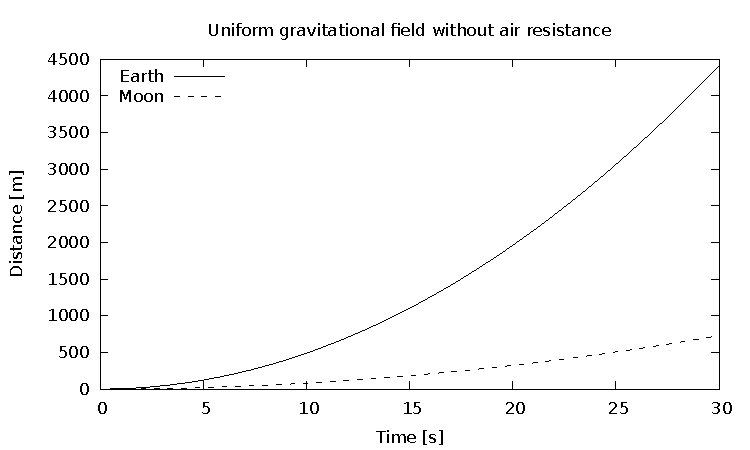
\includegraphics{gnuplot-bw}
 	\caption{Černobílá varianta obrázku generovaného programem Gnuplot}\label{fig:gnuplot-bw}
 \end{figure}
 
 \begin{figure}\centering
 	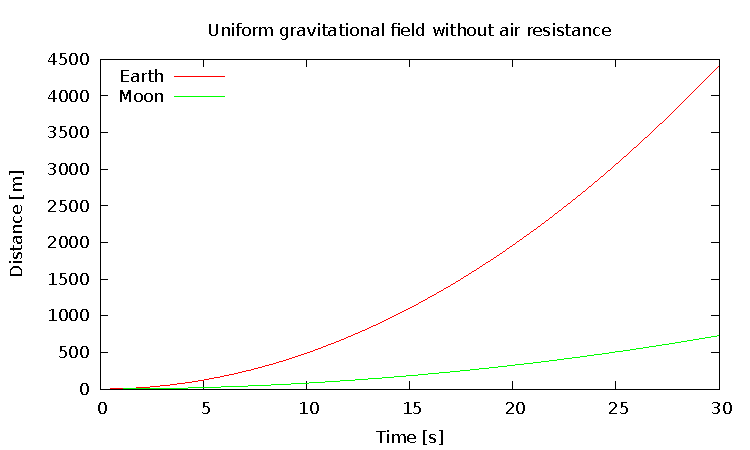
\includegraphics{gnuplot-col}
 	\caption{Barevná varianta obrázku generovaného programem Gnuplot}\label{fig:gnuplot-col}
 \end{figure}
 
 
 \subsection{Tabulky}
 
 Tabulky lze zadávat různě, např. v~prostředí \verb|tabular|, avšak pro jejich vkládání platí to samé, co pro obrázky -- použijte plovoucí prostředí, v~tomto případě \verb|table|. Například tabulka \ref{tab:matematika} byla vložena tímto způsobem.
 
 \begin{table}\centering
 	\caption[Příklad tabulky]{Zadávání matematiky}\label{tab:matematika}
 	\begin{tabular}{|l|l|c|c|}\hline
 		Typ		& Prostředí		& \LaTeX{}ovská zkratka	& \TeX{}ovská zkratka	\tabularnewline \hline \hline
 		Text		& \verb|math|		& \verb|\(...\)|	& \verb|$...$|		\tabularnewline \hline
 		Displayed	& \verb|displaymath|	& \verb|\[...\]|	& \verb|$$...$$|	\tabularnewline \hline
 	\end{tabular}
 \end{table}
 
% % % % % % % % % % % % % % % % % % % % % % % % % % % % 

\chapter{Obsah přiloženého CD}

\end{document}
